% ============================================================
%  يُترجَم بـ XeLaTeX  (في Overleaf: Menu → Compiler → XeLaTeX)
%  الخط: Amiri (متوفر في Overleaf، أو حمّله من github.com/aliftype/amiri)
% ============================================================
\documentclass[12pt,a4paper]{article}
\usepackage[a4paper,margin=1.7cm,top=2.3cm,bottom=2.9cm,headheight=15pt,footskip=1.5cm]{geometry}
\usepackage{amsmath,amssymb}
\usepackage{icomma}
\usepackage[english,bidi=default,layout=lists]{babel}
\babelprovide[import,main]{arabic}
\babelfont{rm}[Scale=1.08]{Amiri}
\babelfont{sf}[Scale=1.08]{Amiri}
\usepackage[most]{tcolorbox}
\usepackage{tikz}
\usetikzlibrary{arrows.meta,calc,shadings}
\usepackage{array}
\usepackage{colortbl}
\usepackage{fancyhdr}
\usepackage{titlesec}
\usepackage{enumitem}
\usepackage{collcell}
\usepackage{needspace}
\usepackage{etoolbox}
\newcolumntype{C}{>{\collectcell\ar}c<{\endcollectcell}}
\pretocmd{\section}{\Needspace{15\baselineskip}}{}{}
\pretocmd{\subsection}{\Needspace{11\baselineskip}}{}{}

\definecolor{cDef}{HTML}{1F4E9C}
\definecolor{cThm}{HTML}{B3261E}
\definecolor{cRem}{HTML}{2E7D32}
\definecolor{cEx}{HTML}{C76B00}
\definecolor{cMeth}{HTML}{6A1B9A}
\definecolor{cSol}{HTML}{00695C}
\definecolor{cSec}{HTML}{1F3A68}

\titleformat{\section}{\Large\bfseries\color{cSec}}{\thesection.}{0.6em}{}[{\color{cSec!60}\titlerule[1pt]}]
\titleformat{\subsection}{\large\bfseries\color{cThm!85!black}}{\thesubsection.}{0.5em}{}
\titlespacing*{\section}{0pt}{14pt}{8pt}
\titlespacing*{\subsection}{0pt}{10pt}{5pt}
\setlength{\parindent}{0pt}
\setlength{\parskip}{4pt}
\setlist{itemsep=2pt,topsep=3pt}

\newtcolorbox{arbox}[3][]{enhanced,
  colback=#2!5,colframe=#2!80!black,arc=2mm,boxrule=0.8pt,
  left=6pt,right=6pt,top=8pt,bottom=5pt,
  fonttitle=\bfseries,coltitle=white,
  title={\foreignlanguage{arabic}{#3}},
  attach boxed title to top right={xshift=-5mm,yshift=-3mm},
  boxed title style={colback=#2!80!black,arc=1.5mm,boxrule=0pt},
  before upper={\selectlanguage{arabic}},
  before skip=8pt,after skip=8pt,breakable,#1}
\newenvironment{BOX}[2]{\begin{otherlanguage}{english}\begin{arbox}{#1}{#2}}{\end{arbox}\end{otherlanguage}}
\newenvironment{tarif}[1][تعريف]{\begin{BOX}{cDef}{#1}}{\end{BOX}}
\newenvironment{khassia}[1][خاصية]{\begin{BOX}{cThm}{#1}}{\end{BOX}}
\newenvironment{molahada}[1][ملاحظة]{\begin{BOX}{cRem}{#1}}{\end{BOX}}
\newenvironment{mithal}[1][مثال]{\begin{BOX}{cEx}{#1}}{\end{BOX}}
\newenvironment{tariqa}[1][طريقة]{\begin{BOX}{cMeth}{#1}}{\end{BOX}}

\newcounter{exo}
\newenvironment{tamrin}[1]{\stepcounter{exo}\begin{BOX}{cSec}{التمرين \theexo: #1}}{\end{BOX}}
\newenvironment{hal}{\Needspace{12\baselineskip}\begin{otherlanguage}{english}\begin{arbox}[breakable]{cSol}{حل التمرين \theexo}}{\end{arbox}\end{otherlanguage}}

\newenvironment{LTR}{\begin{otherlanguage}{english}}{\end{otherlanguage}}
\newcommand{\ar}[1]{\foreignlanguage{arabic}{#1}}

\renewcommand{\dots}{\mathinner{\ldotp\ldotp\ldotp}}
\renewcommand{\ldots}{\mathinner{\ldotp\ldotp\ldotp}}
\renewcommand{\cdots}{\mathinner{\cdotp\cdotp\cdotp}}
\newcommand{\N}{\mathbb{N}}
\newcommand{\Z}{\mathbb{Z}}
\newcommand{\D}{\mathbb{D}}
\newcommand{\Q}{\mathbb{Q}}
\newcommand{\R}{\mathbb{R}}
\newcommand{\pgcd}{\operatorname{PGCD}}
\newcommand{\ppcm}{\operatorname{PPCM}}

% \NLseg{a}{b}{[}{]} ; \NLright{a}{[} ; \NLleft{b}{]}  (interval on a number line)
\newcommand{\NLseg}[4]{\begin{LTR}\begin{tikzpicture}[baseline=-0.6ex]
 \draw[-{Stealth[length=2mm]},gray!70](0,0)--(3.4,0);
 \draw[line width=2pt,cThm!80!black](0.7,0)--(2.7,0);
 \node[cThm!80!black,font=\LARGE] at (0.7,0){$#3$};
 \node[cThm!80!black,font=\LARGE] at (2.7,0){$#4$};
 \node[below=3pt,font=\footnotesize] at (0.7,0){$#1$};
 \node[below=3pt,font=\footnotesize] at (2.7,0){$#2$};
\end{tikzpicture}\end{LTR}}
\newcommand{\NLright}[2]{\begin{LTR}\begin{tikzpicture}[baseline=-0.6ex]
 \draw[-{Stealth[length=2mm]},gray!70](0,0)--(3.4,0);
 \draw[line width=2pt,cThm!80!black](1.3,0)--(3.3,0);
 \node[cThm!80!black,font=\LARGE] at (1.3,0){$#2$};
 \node[below=3pt,font=\footnotesize] at (1.3,0){$#1$};
\end{tikzpicture}\end{LTR}}
\newcommand{\NLleft}[2]{\begin{LTR}\begin{tikzpicture}[baseline=-0.6ex]
 \draw[-{Stealth[length=2mm]},gray!70](0,0)--(3.4,0);
 \draw[line width=2pt,cThm!80!black](0.05,0)--(2.1,0);
 \node[cThm!80!black,font=\LARGE] at (2.1,0){$#2$};
 \node[below=3pt,font=\footnotesize] at (2.1,0){$#1$};
\end{tikzpicture}\end{LTR}}

% ---------- social-media icons (pure TikZ) ----------
\definecolor{cFB}{HTML}{1877F2}
\definecolor{cTG}{HTML}{229ED9}
\definecolor{cIG1}{HTML}{FEDA75}
\definecolor{cIG2}{HTML}{D62976}
\definecolor{cIG3}{HTML}{4F5BD5}
\newcommand{\fbicon}{\begin{LTR}\begin{tikzpicture}[baseline=-0.75ex,x=1em,y=1em]
 \fill[cFB] (0,0) circle (0.55);
 \node[white,inner sep=0,font=\usefont{TU}{lmss}{bx}{n}\small] at (0.04,-0.02) {f};
\end{tikzpicture}\end{LTR}}
\newcommand{\igicon}{\begin{LTR}
\begin{tikzpicture}[baseline=-0.75ex,x=1em,y=1em]
 \shade[lower left=cIG1,lower right=cIG2,upper left=cIG2,upper right=cIG3,rounded corners=0.28em] (-0.55,-0.55) rectangle (0.55,0.55);
 \draw[white,line width=0.09em,rounded corners=0.18em] (-0.36,-0.36) rectangle (0.36,0.36);
 \draw[white,line width=0.09em] (0,0) circle (0.17);
 \fill[white] (0.22,0.22) circle (0.05);
\end{tikzpicture}\end{LTR}}
\newcommand{\tgicon}{\begin{LTR}
\begin{tikzpicture}[baseline=-0.75ex,x=1em,y=1em]
 \fill[cTG] (0,0) circle (0.55);
 \fill[white] (-0.33,0.0) -- (0.32,0.27) -- (0.2,-0.3) -- (0.0,-0.15) -- (-0.08,-0.28) -- (-0.08,-0.08) -- cycle;
 \fill[cTG!70!black] (-0.08,-0.08) -- (0.25,0.2) -- (0.0,-0.15) -- (-0.08,-0.28) -- cycle;
\end{tikzpicture}\end{LTR}}
% page number: black box, white two-digit number, at the right of the social row
\newcommand{\PageBox}{\begin{LTR}\tikz[baseline=(p.base)]\node[fill=black,text=white,inner sep=2.5pt,minimum width=1.6em,minimum height=1.3em,font=\usefont{TU}{lmss}{bx}{n}\small](p){\ifnum\value{page}<10 0\fi\arabic{page}};\end{LTR}}
% visual left-to-right order: Telegram | Instagram | Facebook | page box
\newcommand{\SocialRow}{\begin{otherlanguage}{english}%
 \ar{\textbf{الأستاذ سوايسية هشام للرياضيات}}\ \tgicon\hfill
 \textbf{prof\_hicham\_math}\ \igicon\hfill
 \ar{\textbf{الأستاذ سوايسية هشام للرياضيات}}\ \fbicon\hspace{2.2em}\PageBox\end{otherlanguage}}

\pagestyle{fancy}
\fancyhf{}
\renewcommand{\headrulewidth}{0.6pt}
\renewcommand{\footrulewidth}{0.4pt}
% \SetHeader{right head: document title}{left head: level -- stream}
\newcommand{\SetHeader}[2]{%
 \fancyhead[C]{\parbox{\textwidth}{\ar{#1\hfill #2}}}%
 \fancyfoot[C]{\parbox{\textwidth}{\small\SocialRow}}}
\usepackage{tkz-tab}
\usepackage{multicol}
% variation / sign table (LTR)
\newenvironment{TAB}{\par\begin{center}\begin{LTR}\begin{tikzpicture}[scale=0.95,every node/.style={font=\small}]}{\end{tikzpicture}\end{LTR}\end{center}}
% grid + axes, clipped: \begin{GR}{xmin}{xmax}{ymin}{ymax}{unit cm}
\newenvironment{GR}[5]{\par\begin{center}\begin{LTR}\begin{tikzpicture}[x=#5cm,y=#5cm,font=\footnotesize]
 \draw[gray!25,very thin] (#1,#3) grid (#2,#4);
 \draw[-{Stealth[length=2mm]}] (#1,0)--(#2+0.3,0) node[below left]{$x$};
 \draw[-{Stealth[length=2mm]}] (0,#3)--(0,#4+0.3) node[below left]{$y$};
 \node[below left] at (0,0){$O$};
 \begin{scope}\clip (#1,#3) rectangle (#2,#4);}
{\end{scope}\end{tikzpicture}\end{LTR}\end{center}}
\newcommand{\Ticks}[2]{\foreach \t in {#1} \node[below,font=\scriptsize] at (\t,0){$\t$}; \foreach \t in {#2} \node[left,font=\scriptsize] at (0,\t){$\t$};}
\newcommand{\bx}[1]{\ensuremath{\colorbox{cDef!12}{$\displaystyle #1$}}}
\newcommand{\TwoCol}[4]{\par\begin{LTR}\noindent\begin{minipage}[t]{#1\textwidth}\selectlanguage{arabic}#2\end{minipage}\hfill\begin{minipage}[t]{#3\textwidth}\selectlanguage{arabic}#4\end{minipage}\end{LTR}\par}
\newcommand{\RL}[4]{\TwoCol{#3}{#4}{#1}{#2}}  % \RL{w1}{right content}{w2}{left content}
\newcommand{\ok}{$\textcolor{cRem}{\checkmark}$}
\newcommand{\limn}{\displaystyle\lim_{n\to+\infty}}
% sub-questions, each on its own line
\newenvironment{sq}{\begin{itemize}[leftmargin=2.4em,itemsep=3pt]}{\end{itemize}}
\newcommand{\qa}{\item[(أ)]}\newcommand{\qb}{\item[(ب)]}\newcommand{\qc}{\item[(جـ)]}\newcommand{\qd}{\item[(د)]}\newcommand{\qe}{\item[(هـ)]}
\newcommand{\pa}{\par\smallskip\textbf{(أ)} }\newcommand{\pb}{\par\smallskip\textbf{(ب)} }\newcommand{\pc}{\par\smallskip\textbf{(جـ)} }\newcommand{\pd}{\par\smallskip\textbf{(د)} }\newcommand{\pe}{\par\smallskip\textbf{(هـ)} }
\newcommand{\QQ}[1]{\par\smallskip\textbf{#1.} }
\newenvironment{tmr}{\stepcounter{exo}\begin{BOX}{cSec}{تمرين محلول \theexo}}{\end{BOX}}
\newcommand{\ABC}[3]{\\[2pt]\begin{tabular}{p{0.28\textwidth}p{0.28\textwidth}p{0.28\textwidth}}(جـ) \ #3 & (ب) \ #2 & (أ) \ #1\end{tabular}}
\pretocmd{\section}{\Needspace{24\baselineskip}}{}{}
\newtcbox{\bxtbox}{on line,colback=cDef!12,colframe=cDef!12,boxrule=0pt,arc=1pt,boxsep=0pt,left=2pt,right=2pt,top=1pt,bottom=1pt}
\newcommand{\bxt}[1]{\foreignlanguage{english}{\bxtbox{\ar{#1}}}}
\usepackage{longtable}
\setlength{\LTpre}{4pt}\setlength{\LTpost}{0pt}
\newcommand{\Phase}[1]{\textbf{#1}}
\newcommand{\Fld}[2]{\textbf{#1:}\ #2}
% رأس المذكرة على نمط النموذج: إطار بعنوان «مذكرة رقم»، معلومات الحصة، ثم إطار الكفاءات
\newcommand{\ModhHead}[9]{%
\begin{LTR}
\begin{tcolorbox}[enhanced,colback=white,colframe=cThm!85!black,arc=4mm,boxrule=1pt,top=14pt,bottom=6pt,left=8pt,right=8pt,
 overlay={\node[fill=cThm!85!black,text=white,rounded corners=3mm,inner xsep=14pt,inner ysep=4pt,font=\large\bfseries] at ([yshift=0pt]frame.north){\ar{مذكرة رقم #1}};},
 before upper={\selectlanguage{arabic}}]
\begin{tabular}{@{}p{0.4\linewidth}p{0.55\linewidth}@{}}
\Fld{المستوى}{#2} & \Fld{الثانوية}{\dotfill}\\[3pt]
\Fld{المادة}{رياضيات} & \Fld{ميدان التعلم}{#3}\\[3pt]
\Fld{المدة}{#5} & \Fld{الوحدة التعلمية}{#4}\\[3pt]
\Fld{الأستاذ}{\dotfill} & \Fld{المحتوى المعرفي}{#6}\\
\end{tabular}
\end{tcolorbox}
\begin{tcolorbox}[enhanced,colback=white,colframe=cThm!85!black,arc=3mm,boxrule=0.8pt,sidebyside,sidebyside align=top,lefthand ratio=0.5,
 segmentation style={dashed,cThm!60},before upper={\selectlanguage{arabic}},before lower={\selectlanguage{arabic}}]
\textbf{الكفاءات المستهدفة:}\par #8
\tcblower
\textbf{الكفاءات القبلية:}\par #7
\end{tcolorbox}
\end{LTR}
\par\smallskip\textbf{الوسائل:} #9\par\smallskip}
\newenvironment{Sayr}{%
\begin{LTR}\renewcommand{\arraystretch}{1.25}
\begin{longtable}{|p{0.17\textwidth}|>{\centering\arraybackslash}p{0.06\textwidth}|p{0.53\textwidth}|>{\centering\arraybackslash}p{0.12\textwidth}|}
\hline\rowcolor{cThm!12}\ar{\textbf{توجيهات وتعاليق}} & \ar{\textbf{المدة}} & \ar{\textbf{سير الحصة}} & \ar{\textbf{مراحل الحصة}}\\\hline\endhead
\hline\endfoot}{\end{longtable}\end{LTR}}
% سطر في الجدول: \Row{مرحلة}{سير}{مدة}{توجيهات}
\newcommand{\Row}[4]{\ar{\small #4} & \ar{#3} & \ar{#2} & \cellcolor{cThm!8}\ar{\Phase{#1}}\\\hline}

\newcommand{\Lab}[2]{\foreignlanguage{english}{\tcbox[on line,colback=#1,colframe=#1,boxrule=0pt,arc=2pt,boxsep=1pt,left=5pt,right=5pt,top=1pt,bottom=1pt]{\ar{\textcolor{white}{\textbf{#2}}}}}}
\newcommand{\Num}[1]{\foreignlanguage{english}{\tikz[baseline=(c.base)]\node[fill=cDef,text=white,inner sep=2pt,font=\footnotesize\bfseries](c){#1};}}
\newcommand{\ck}{\ensuremath{{\color{cRem}\checkmark}}}
\newenvironment{Kad}[1]{\par\smallskip\Lab{#1}}{\par}
\SetHeader{\small\bfseries\color{cSec}مذكرات محور: الاشتقاقية}{\small\color{cSec}السنة الثانية ثانوي -- علوم تجريبية}
\begin{document}
\begin{LTR}
\begin{tcolorbox}[enhanced,colback=cThm!85!black,colframe=cThm!85!black,arc=3mm,halign=center,boxrule=0pt,top=12pt,bottom=12pt,before upper={\selectlanguage{arabic}}]
{\color{white}\fontsize{26}{32}\selectfont\bfseries مذكرات محور: الاشتقاقية}\\[8pt]
{\color{white}\large السنة الثانية ثانوي -- علوم تجريبية (صالحة لشعبتي رياضيات وتقني رياضي)}\\[4pt]
{\color{white}\large 8 مذكرات (16 ساعة) -- السنة الدراسية 2026-2027}
\end{tcolorbox}
\end{LTR}
\begin{BOX}{cThm}{يتضمن هذا العمل}
\begin{enumerate}[label=\textbf{مذكرة \arabic{enumi}:},leftmargin=6em,start=10]
\item العدد المشتق لدالة عند عدد حقيقي.
\item التفسير الهندسي للعدد المشتق: المماس.
\item التقريب التآلفي لدالة.
\item الدالة المشتقة ومشتقات الدوال المألوفة.
\item العمليات على الدوال المشتقة.
\item المشتق واتجاه التغير.
\item القيم الحدية المحلية لدالة.
\item تطبيقات الاشتقاقية: حل مسائل بدوال ناطقة.
\end{enumerate}
مراجع النشاطات والتمارين: الكتاب المدرسي للسنة الثانية ثانوي (باب الاشتقاقية ص 62 و 83--87 ، باب تطبيقات الاشتقاقية ص 92 و 98 و 104--107).
\end{BOX}
\newpage
\ModhHead{10}{2 ع ت}{تحليل}{الاشتقاقية}{02 سا}{العدد المشتق لدالة عند عدد حقيقي}%
{\begin{itemize}\item الدوال ، نسبة التزايد (1 ج م).\item معامل توجيه مستقيم.\end{itemize}}%
{\begin{itemize}\item حساب نهاية بسيطة عند $0$.\item دراسة قابلية اشتقاق دالة عند عدد وحساب العدد المشتق.\end{itemize}}%
{المنهاج ، الكتاب المدرسي ، مراجع ، الحاسبة البيانية.}
\begin{Sayr}
\Row{مرحلة الانطلاق}{%
\textbf{التهيئة النفسية:} سيارة تقطع $100$ km في ساعتين: هل سرعتها في كل لحظة $50$ km/h ؟ ماذا يقيس العداد؟}{10 د}{سؤال من الحياة.}
\Row{التشخيص والاكتشاف}{%
\Lab{cEx}{مناقشة نشاط 01 صفحة 62}\par\ck\ السرعة المتوسطة بين اللحظتين $2$ و $2+h$: $v_m=\dfrac{d(2+h)-d(2)}h$.\par
\ck\ جدول قيم لـ $v_m$ من أجل $h$ قريب من $0$: القيم تقترب من عدد ثابت هو \textbf{السرعة اللحظية}.\par
}{35 د}{جدول قيم بالحاسبة.}
\Row{بناء المعارف}{%
\Lab{cDef}{نهاية عند الصفر}\ نقول إن $f(h)$ يؤول إلى $l$ لما يؤول $h$ إلى $0$ إذا أمكن جعل $f(h)$ قريباً من $l$ بالقدر الذي نريد ، ونكتب $\lim\limits_{h\to0}f(h)=l$.\par\Lab{cEx}{مثال}\ $\lim\limits_{h\to0}(3h^2-h+2)=2$ ؛ $\lim\limits_{h\to0}\dfrac{h^2+5h}h=\lim\limits_{h\to0}(h+5)=5$.\par}{50 د}{نكتب خطوات الحساب الثلاث.}
\Row{}{%
\Lab{cDef}{العدد المشتق}\ $f$ قابلة للاشتقاق عند $x_0$ إذا كانت نسبة التزايد $\dfrac{f(x_0+h)-f(x_0)}h$ تقبل نهاية حقيقية $l$ لما يؤول $h$ إلى $0$ ؛ نسميها العدد المشتق ونرمز لها $f^{\prime}(x_0)$.\par\Lab{cEx}{مثال}\ $f(x)=x^2$ ، $x_0=3$: $\dfrac{(3+h)^2-9}h=6+h$ ، إذن $f^{\prime}(3)=6$.\par}{}{}
\Row{}{%
\Lab{cThm!80!black}{حذار}\ لا نعوض $h=0$ مباشرة في النسبة (حالة $\frac00$): نبسط أولاً.}{}{}
\Row{التقويم}{%
\Lab{cEx}{تطبيق}\par $f(x)=x^2+x$. احسب نسبة التزايد بين $2$ و $2+h$ ، ثم استنتج $f^{\prime}(2)$.\par\textbf{الحل:} $\dfrac{(2+h)^2+(2+h)-6}h=\dfrac{h^2+5h}h=h+5$ ، إذن $f^{\prime}(2)=5$.\par\textbf{واجب منزلي:} تمارين 22 إلى 26 صفحة 83.\par\smallskip\textbf{ملاحظات حول سير الحصة:} \dotfill}{25 د}{تقويم فردي.}
\end{Sayr}
\newpage
\ModhHead{11}{2 ع ت}{تحليل}{الاشتقاقية}{02 سا}{التفسير الهندسي للعدد المشتق: المماس}%
{\begin{itemize}\item العدد المشتق ، معادلة مستقيم.\end{itemize}}%
{\begin{itemize}\item كتابة معادلة المماس لمنحنٍ عند نقطة منه.\end{itemize}}%
{المنهاج ، الكتاب المدرسي ، مراجع ، الحاسبة البيانية.}
\begin{Sayr}
\Row{مرحلة الانطلاق}{%
\textbf{التهيئة النفسية:} ما معامل توجيه المستقيم المار بالنقطتين $A(1;2)$ و $B(3;8)$ ؟}{10 د}{تذكير.}
\Row{التشخيص والاكتشاف}{%
\Lab{cEx}{مناقشة نشاط 02 صفحة 62}\par\ck\ النقطة $M$ تقترب من $L$ على المنحني: معامل توجيه $(LM)$ هو نسبة التزايد.\par
\ck\ لما يؤول $h$ إلى $0$ يصبح $(LM)$ \textbf{مماساً} للمنحني ، ومعامل توجيهه العدد المشتق.\par
}{35 د}{نحرك النقطة على الحاسبة البيانية.}
\Row{بناء المعارف}{%
\Lab{cDef}{تعريف}\ إذا كانت $f$ قابلة للاشتقاق عند $x_0$ ، فالمماس لـ $C_f$ عند $A\big(x_0;f(x_0)\big)$ هو المستقيم الذي يشمل $A$ ومعامل توجيهه $f^{\prime}(x_0)$.\par\Lab{cThm}{معادلة المماس}\ $y=f^{\prime}(x_0)(x-x_0)+f(x_0)$.\par}{50 د}{نرسم المماس بدقة.}
\Row{}{%
\Lab{cEx}{مثال}\ $f(x)=x^2-2x$ عند $x_0=3$: $f(3)=3$ ؛ $\dfrac{f(3+h)-f(3)}h=h+4$ ، إذن $f^{\prime}(3)=4$ ، والمماس $y=4(x-3)+3=4x-9$.\par\smallskip\begin{LTR}\centering 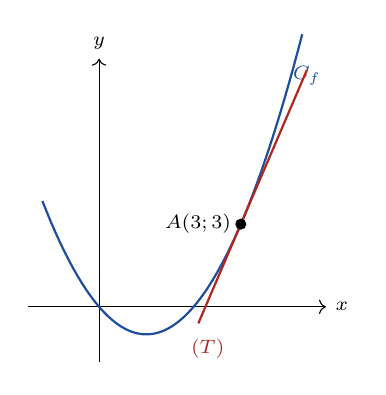
\begin{tikzpicture}[x=0.6cm,y=0.35cm,font=\scriptsize]
\draw[->] (-1.5,0)--(4.8,0) node[right]{$x$}; \draw[->] (0,-2)--(0,9) node[above]{$y$};
\draw[cDef,thick,domain=-1.2:4.3,samples=60] plot (\x,{\x*\x-2*\x}); \node[cDef] at (4.4,8.4){$C_f$};
\draw[cThm,thick,domain=2.1:4.4] plot (\x,{4*\x-9}); \node[cThm] at (2.3,-1.5){$(T)$};
\fill (3,3) circle (2pt) node[left]{$A(3;3)$};
\end{tikzpicture}\end{LTR}\par \Lab{cRem}{ملاحظات}\ إذا كان $f^{\prime}(x_0)=0$ فالمماس موازٍ لمحور الفواصل.}{}{}
\Row{التقويم}{%
\Lab{cEx}{تطبيق}\par اكتب معادلة المماس لمنحني $f(x)=\dfrac1x$ عند النقطة ذات الفاصلة $2$.\par\textbf{الحل:} $\dfrac{f(2+h)-f(2)}h=\dfrac{-1}{2(2+h)}$ ، إذن $f^{\prime}(2)=-\dfrac14$ ؛ $f(2)=\dfrac12$ ؛ المماس: $y=-\dfrac14x+1$.\par\textbf{واجب منزلي:} تمارين 34 ، 35 ، 36 صفحة 84 ، وتمارين 49 إلى 53 صفحة 84.\par\smallskip\textbf{ملاحظات حول سير الحصة:} \dotfill}{25 د}{تقويم فردي.}
\end{Sayr}
\newpage
\ModhHead{12}{2 ع ت}{تحليل}{الاشتقاقية}{02 سا}{التقريب التآلفي لدالة}%
{\begin{itemize}\item العدد المشتق ، معادلة المماس.\end{itemize}}%
{\begin{itemize}\item تعيين التقريب التآلفي لدالة عند عدد ، واستعماله لحساب قيم مقربة.\end{itemize}}%
{المنهاج ، الكتاب المدرسي ، مراجع ، الحاسبة البيانية.}
\begin{Sayr}
\Row{مرحلة الانطلاق}{%
\textbf{التهيئة النفسية:} بدون حاسبة: ما قيمة تقريبية لـ $\sqrt{1{,}0004}$ ؟}{10 د}{تحدٍّ ذهني.}
\Row{التشخيص والاكتشاف}{%
\Lab{cEx}{وضعية مقترحة}\ $f(x)=\sqrt{1+x}$ و $g(x)=1+\dfrac12x$ (مماس $C_f$ عند $0$). نملأ جدولاً لـ $f(x)$ و $g(x)$ من أجل $x=\pm0{,}001$ ، $\pm0{,}002$.\par\ck\ القيم متقاربة جداً: بالقرب من $0$ ، المنحني «يلتصق» بمماسه.\par
}{35 د}{مقارنة بالحاسبة.}
\Row{بناء المعارف}{%
\Lab{cThm}{خاصية}\ إذا كانت $f$ قابلة للاشتقاق عند $a$ ، فمن أجل $h$ قريب من $0$: $f(a+h)\approx f(a)+f^{\prime}(a)\,h$.\par الدالة $h\mapsto f(a)+f^{\prime}(a)h$ هي \textbf{التقريب التآلفي} لـ $f$ عند $a$.\par\Lab{cEx}{مثال}\par\ck\ $\sqrt{1+h}\approx1+\dfrac h2$: $\sqrt{1{,}0004}\approx1{,}0002$ (الحاسبة: $1{,}00019998$).\par
\ck\ $(1+h)^2\approx1+2h$: $1{,}002^2\approx1{,}004$ (القيمة المضبوطة $1{,}004004$).\par
}{50 د}{نبرز الخطأ المرتكب.}
\Row{}{%
\Lab{cThm!80!black}{حذار}\ التقريب جيد فقط لما يكون $h$ قريباً من $0$.}{}{}
\Row{التقويم}{%
\Lab{cEx}{تطبيق}\par عيّن التقريب التآلفي لـ $f(x)=\dfrac1x$ عند $1$ ، ثم قيمة مقربة لـ $\dfrac1{1{,}003}$.\par\textbf{الحل:} $f(1)=1$ ، $f^{\prime}(1)=-1$: $\dfrac1{1+h}\approx1-h$ ، إذن $\dfrac1{1{,}003}\approx0{,}997$.\par\textbf{واجب منزلي:} تمارين 43 إلى 48 صفحتي 84 و 85.\par\smallskip\textbf{ملاحظات حول سير الحصة:} \dotfill}{25 د}{تقويم فردي.}
\end{Sayr}
\newpage
\ModhHead{13}{2 ع ت}{تحليل}{الاشتقاقية}{02 سا}{الدالة المشتقة ومشتقات الدوال المألوفة}%
{\begin{itemize}\item قابلية الاشتقاق والعدد المشتق.\end{itemize}}%
{\begin{itemize}\item تعيين الدالة المشتقة لدالة على مجال.\item معرفة مشتقات الدوال المألوفة.\end{itemize}}%
{المنهاج ، الكتاب المدرسي ، مراجع ، الحاسبة البيانية.}
\begin{Sayr}
\Row{مرحلة الانطلاق}{%
\textbf{التهيئة النفسية:} احسب $f^{\prime}(1)$ ، $f^{\prime}(2)$ ، $f^{\prime}(3)$ للدالة $f(x)=x^2$: هل تلاحظ قاعدة؟}{10 د}{سؤال تمهيدي.}
\Row{التشخيص والاكتشاف}{%
\Lab{cEx}{وضعية مقترحة}\ نحسب نسبة التزايد عند عدد كيفي $x$:\par\ck\ $f(x)=x^2$: $\dfrac{(x+h)^2-x^2}h=2x+h$ ، إذن $f^{\prime}(x)=2x$.\par
\ck\ $f(x)=\dfrac1x$: $\dfrac{\frac1{x+h}-\frac1x}h=\dfrac{-1}{x(x+h)}$ ، إذن $f^{\prime}(x)=-\dfrac1{x^2}$.\par
}{35 د}{عمل ثنائي.}
\Row{بناء المعارف}{%
\Lab{cDef}{تعريف}\ إذا كانت $f$ قابلة للاشتقاق عند كل $x$ من مجال $I$ ، فالدالة $x\mapsto f^{\prime}(x)$ هي \textbf{الدالة المشتقة} لـ $f$ على $I$.\par\Lab{cThm}{مشتقات الدوال المألوفة}\par\smallskip\begin{LTR}\centering {\footnotesize\renewcommand{\arraystretch}{1.5}\begin{tabular}{|c|c|c|}\hline
\rowcolor{cSec!12}$f(x)$ & $f^{\prime}(x)$ & \ar{مجال قابلية الاشتقاق}\\\hline
$k$ & $0$ & $\mathbb R$\\\hline
$x$ & $1$ & $\mathbb R$\\\hline
$x^n\ (n\geqslant2)$ & $nx^{n-1}$ & $\mathbb R$\\\hline
$\dfrac1x$ & $-\dfrac1{x^2}$ & $]-\infty;0[$ \ar{أو} $]0;+\infty[$\\\hline
$\sqrt x$ & $\dfrac1{2\sqrt x}$ & $]0;+\infty[$\\\hline
\end{tabular}}\end{LTR}\par }{50 د}{الجدول يُحفظ.}
\Row{}{%
\Lab{cThm!80!black}{حذار}\ الدالة $\sqrt x$ معرفة عند $0$ لكنها غير قابلة للاشتقاق عنده.\par\Lab{cEx}{مثال}\ $f(x)=x^5$: $f^{\prime}(x)=5x^4$ ؛ $g(x)=\sqrt x$: $g^{\prime}(4)=\dfrac14$.}{}{}
\Row{التقويم}{%
\Lab{cEx}{تطبيق}\par احسب $f^{\prime}(x)$ في كل حالة: $f(x)=x^3$ ؛ $f(x)=7$ ؛ ثم $f^{\prime}(-2)$ للدالة $f(x)=\dfrac1x$.\par\textbf{الحل:} $3x^2$ ؛ $0$ ؛ $-\dfrac14$.\par\textbf{واجب منزلي:} تمارين 38 ، 39 ، 40 صفحة 84 (دون استعمال التعريف).\par\smallskip\textbf{ملاحظات حول سير الحصة:} \dotfill}{25 د}{تقويم فردي.}
\end{Sayr}
\newpage
\ModhHead{14}{2 ع ت}{تحليل}{الاشتقاقية}{02 سا}{العمليات على الدوال المشتقة}%
{\begin{itemize}\item مشتقات الدوال المألوفة.\end{itemize}}%
{\begin{itemize}\item حساب مشتقات $u+v$ ، $ku$ ، $uv$ ، $\frac1v$ ، $\frac uv$ ، $f(ax+b)$.\end{itemize}}%
{المنهاج ، الكتاب المدرسي ، مراجع ، الحاسبة البيانية.}
\begin{Sayr}
\Row{مرحلة الانطلاق}{%
\textbf{التهيئة النفسية:} هل مشتق الجداء هو جداء المشتقين؟ جرّب مع $x\times x$.}{10 د}{تحدٍّ.}
\Row{التشخيص والاكتشاف}{%
\Lab{cEx}{وضعية مقترحة}\ $u(x)=x+1$ ، $v(x)=x-2$.\par\ck\ $(u\times v)(x)=x^2-x-2$ ، مشتقها $2x-1$ ؛ بينما $u^{\prime}\times v^{\prime}=1$.\par
\ck\ نتحقق أن $u^{\prime}v+uv^{\prime}=(x-2)+(x+1)=2x-1$.\par
}{35 د}{كشف الخطأ الشائع.}
\Row{بناء المعارف}{%
\Lab{cThm}{خاصية}\ $u$ و $v$ قابلتان للاشتقاق على $I$ ($v$ لا تنعدم على $I$ في حالة القسمة):\par\smallskip\begin{LTR}\centering {\footnotesize\renewcommand{\arraystretch}{1.6}\begin{tabular}{|c|c|}\hline
\rowcolor{cSec!12}\ar{الدالة} & \ar{مشتقتها}\\\hline
$u+v$ & $u^{\prime}+v^{\prime}$\\\hline
$ku$ & $ku^{\prime}$\\\hline
$u\times v$ & $u^{\prime}v+uv^{\prime}$\\\hline
$\dfrac1v$ & $-\dfrac{v^{\prime}}{v^2}$\\\hline
$\dfrac uv$ & $\dfrac{u^{\prime}v-uv^{\prime}}{v^2}$\\\hline
$x\mapsto f(ax+b)$ & $x\mapsto a\,f^{\prime}(ax+b)$\\\hline
\end{tabular}}\end{LTR}\par \Lab{cEx}{مثال}\par\ck\ $f(x)=\dfrac{2x+1}{x-1}$: $f^{\prime}(x)=\dfrac{2(x-1)-(2x+1)}{(x-1)^2}=\dfrac{-3}{(x-1)^2}$.\par
\ck\ $g(x)=\sqrt{2x+4}$: $g^{\prime}(x)=2\times\dfrac1{2\sqrt{2x+4}}=\dfrac1{\sqrt{2x+4}}$ على $]-2;+\infty[$.\par
}{50 د}{جدول القواعد يُحفظ.}
\Row{}{%
\Lab{cThm!80!black}{حذار}\ $(uv)^{\prime}\neq u^{\prime}v^{\prime}$ و $\left(\dfrac uv\right)^{\prime}\neq\dfrac{u^{\prime}}{v^{\prime}}$.}{}{}
\Row{التقويم}{%
\Lab{cEx}{تطبيق}\par احسب مشتقة $h(x)=(x^2+1)(x-3)$ بطريقتين (الجداء ، ثم بعد النشر).\par\textbf{الحل:} $h^{\prime}(x)=2x(x-3)+(x^2+1)=3x^2-6x+1$ ؛ وبالنشر $h(x)=x^3-3x^2+x-3$ نجد نفس النتيجة.\par\textbf{واجب منزلي:} تمارين 62 إلى 69 صفحتي 86 و 87.\par\smallskip\textbf{ملاحظات حول سير الحصة:} \dotfill}{25 د}{تقويم فردي.}
\end{Sayr}
\newpage
\ModhHead{15}{2 ع ت}{تحليل}{الاشتقاقية}{02 سا}{المشتق واتجاه التغير}%
{\begin{itemize}\item حساب المشتقات ، إشارة عبارة.\end{itemize}}%
{\begin{itemize}\item استعمال إشارة المشتقة لتعيين اتجاه تغير دالة وتشكيل جدول تغيراتها.\end{itemize}}%
{المنهاج ، الكتاب المدرسي ، مراجع ، الحاسبة البيانية.}
\begin{Sayr}
\Row{مرحلة الانطلاق}{%
\textbf{التهيئة النفسية:} على منحنٍ متزايد ، ماذا تلاحظ عن ميل المماسات؟}{10 د}{ملاحظة بيانية.}
\Row{التشخيص والاكتشاف}{%
\Lab{cEx}{مناقشة نشاط 01 صفحة 92}\par\ck\ رسم مماسات على أجزاء متزايدة ثم متناقصة: معاملات التوجيه موجبة ثم سالبة.\par
\ck\ تخمين العلاقة بين إشارة $f^{\prime}$ واتجاه تغير $f$.\par
}{35 د}{الحاسبة البيانية.}
\Row{بناء المعارف}{%
\Lab{cThm}{خاصية}\ $f$ قابلة للاشتقاق على مجال $I$:\par\ck\ إذا كانت $f^{\prime}(x)>0$ على $I$ (ما عدا عند قيم منعزلة تنعدم فيها) فإن $f$ متزايدة تماماً على $I$.\par
\ck\ إذا كانت $f^{\prime}(x)<0$ على $I$ فإن $f$ متناقصة تماماً على $I$.\par
\ck\ إذا كانت $f^{\prime}(x)=0$ على $I$ فإن $f$ ثابتة على $I$.\par
\Lab{cMeth}{طريقة}\ نحسب $f^{\prime}(x)$ ، ندرس إشارتها ، ثم نشكل جدول التغيرات.\par}{50 د}{جدول التغيرات خطوة خطوة.}
\Row{}{%
\Lab{cEx}{مثال}\ $f(x)=x^3-3x+1$: $f^{\prime}(x)=3x^2-3=3(x-1)(x+1)$ ؛ $f(-1)=3$ ، $f(1)=-1$.\par\smallskip\begin{LTR}\centering 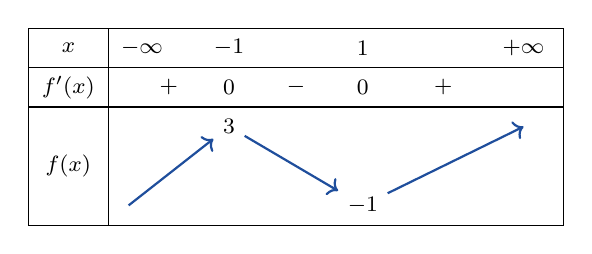
\begin{tikzpicture}[x=0.85cm,y=0.5cm,font=\footnotesize]
\draw (0,0) rectangle (8,-5); \draw (0,-1)--(8,-1); \draw (0,-2)--(8,-2); \draw (1.2,0)--(1.2,-5);
\node at (0.6,-0.5){$x$}; \node at (0.6,-1.5){$f^{\prime}(x)$}; \node at (0.6,-3.5){$f(x)$};
\node at (1.7,-0.5){$-\infty$}; \node at (3,-0.5){$-1$}; \node at (5,-0.5){$1$}; \node at (7.4,-0.5){$+\infty$};
\node at (2.1,-1.5){$+$}; \node at (3,-1.5){$0$}; \node at (4,-1.5){$-$}; \node at (5,-1.5){$0$}; \node at (6.2,-1.5){$+$};
\node (a) at (3,-2.5){$3$}; \node (b) at (5,-4.5){$-1$};
\draw[->,cDef,thick] (1.5,-4.5)--(a); \draw[->,cDef,thick] (a)--(b); \draw[->,cDef,thick] (b)--(7.4,-2.5);
\end{tikzpicture}\end{LTR}\par \Lab{cThm!80!black}{حذار}\ النتيجة صحيحة على \textbf{مجال}.}{}{}
\Row{التقويم}{%
\Lab{cEx}{تطبيق}\par ادرس اتجاه تغير $g(x)=x^2-4x+1$ وشكّل جدول تغيراتها.\par\textbf{الحل:} $g^{\prime}(x)=2x-4$: سالبة على $]-\infty;2]$ وموجبة على $[2;+\infty[$ ؛ $g$ متناقصة ثم متزايدة ، و $g(2)=-3$.\par\textbf{واجب منزلي:} تمارين 22 ، 23 ، 24 ، 29 صفحتي 104 و 105.\par\smallskip\textbf{ملاحظات حول سير الحصة:} \dotfill}{25 د}{تقويم فردي.}
\end{Sayr}
\newpage
\ModhHead{16}{2 ع ت}{تحليل}{الاشتقاقية}{02 سا}{القيم الحدية المحلية لدالة}%
{\begin{itemize}\item المشتق واتجاه التغير.\end{itemize}}%
{\begin{itemize}\item تعيين القيم الحدية المحلية لدالة باستعمال مشتقتها.\end{itemize}}%
{المنهاج ، الكتاب المدرسي ، مراجع ، الحاسبة البيانية.}
\begin{Sayr}
\Row{مرحلة الانطلاق}{%
\textbf{التهيئة النفسية:} في جدول تغيرات المذكرة السابقة: ماذا يمثل العددان $3$ و $-1$ ؟}{10 د}{الرجوع إلى جدول سابق.}
\Row{التشخيص والاكتشاف}{%
\Lab{cEx}{وضعية مقترحة}\ $f(x)=x^2+2x+3$.\par\ck\ $f^{\prime}(x)=2x+2$ تنعدم عند $-1$ مغيرة إشارتها.\par
\ck\ $f(-1)=2$ أصغر قيمة لـ $f$ ؛ والمماس عند $(-1;2)$ أفقي.\par
}{35 د}{عمل ثنائي.}
\Row{بناء المعارف}{%
\Lab{cDef}{تعريف}\ $f(x_0)$ \textbf{قيمة حدية عظمى محلية} إذا وُجد مجال مفتوح $I$ يشمل $x_0$ يكون فيه $f(x)\leqslant f(x_0)$ (وصغرى إذا $f(x)\geqslant f(x_0)$).\par\Lab{cThm}{خاصية}\ إذا انعدمت $f^{\prime}$ عند $x_0$ \textbf{مغيرة إشارتها} فإن $f(x_0)$ قيمة حدية محلية.\par}{50 د}{نبرز شرط تغير الإشارة.}
\Row{}{%
\Lab{cEx}{مثال}\ $f(x)=x+\dfrac1x$ على $\mathbb R^*$: $f^{\prime}(x)=1-\dfrac1{x^2}=\dfrac{(x-1)(x+1)}{x^2}$.\par\smallskip\begin{LTR}\centering 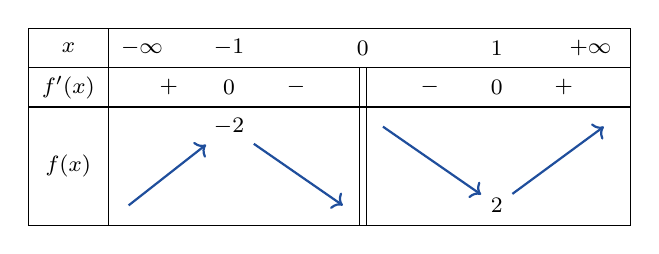
\begin{tikzpicture}[x=0.85cm,y=0.5cm,font=\footnotesize]
\draw (0,0) rectangle (9,-5); \draw (0,-1)--(9,-1); \draw (0,-2)--(9,-2); \draw (1.2,0)--(1.2,-5);
\draw (4.95,-1)--(4.95,-5); \draw (5.05,-1)--(5.05,-5);
\node at (0.6,-0.5){$x$}; \node at (0.6,-1.5){$f^{\prime}(x)$}; \node at (0.6,-3.5){$f(x)$};
\node at (1.7,-0.5){$-\infty$}; \node at (3,-0.5){$-1$}; \node at (5,-0.5){$0$}; \node at (7,-0.5){$1$}; \node at (8.4,-0.5){$+\infty$};
\node at (2.1,-1.5){$+$}; \node at (3,-1.5){$0$}; \node at (4,-1.5){$-$}; \node at (6,-1.5){$-$}; \node at (7,-1.5){$0$}; \node at (8,-1.5){$+$};
\node (a) at (3,-2.5){$-2$}; \node (b) at (7,-4.5){$2$};
\draw[->,cDef,thick] (1.5,-4.5)--(a); \draw[->,cDef,thick] (a)--(4.7,-4.5); \draw[->,cDef,thick] (5.3,-2.5)--(b); \draw[->,cDef,thick] (b)--(8.6,-2.5);
\end{tikzpicture}\end{LTR}\par $f(-1)=-2$ قيمة حدية عظمى محلية ، و $f(1)=2$ قيمة حدية صغرى محلية.\par\Lab{cThm!80!black}{حذار}\ $f(x)=x^3$: $f^{\prime}(0)=0$ لكن $f^{\prime}$ لا تغير إشارتها ، فلا توجد قيمة حدية عند $0$.}{}{}
\Row{التقويم}{%
\Lab{cEx}{تطبيق}\par عيّن القيم الحدية المحلية للدالة $f(x)=x^3-3x+1$ (المذكرة 15).\par\textbf{الحل:} $f^{\prime}$ تنعدم مغيرة إشارتها عند $-1$ و $1$: عظمى محلية $f(-1)=3$ ، صغرى محلية $f(1)=-1$.\par\textbf{واجب منزلي:} تمارين 25 إلى 28 صفحة 104 ، وتمرينا 42 و 43 صفحة 106.\par\smallskip\textbf{ملاحظات حول سير الحصة:} \dotfill}{25 د}{تقويم فردي.}
\end{Sayr}
\newpage
\ModhHead{17}{2 ع ت}{تحليل}{الاشتقاقية}{02 سا}{تطبيقات الاشتقاقية: حل مسائل بدوال ناطقة}%
{\begin{itemize}\item المشتقات ، اتجاه التغير ، المماس.\end{itemize}}%
{\begin{itemize}\item دراسة دالة ناطقة: المشتقة ، التغيرات ، القيم الحدية ، المماس.\item حل مسألة استمثال بسيطة.\end{itemize}}%
{المنهاج ، الكتاب المدرسي ، مراجع ، الحاسبة البيانية.}
\begin{Sayr}
\Row{مرحلة الانطلاق}{%
\textbf{التهيئة النفسية:} بسلك طوله $20$ cm نصنع مستطيلاً: ما أكبر مساحة ممكنة؟}{10 د}{مسألة من الحياة.}
\Row{التشخيص والاكتشاف}{%
\Lab{cEx}{مناقشة أعمال موجهة صفحة 98}\par\ck\ ترييض المسألة بدالة ، ثم دراسة تغيراتها بالمشتقة.\par
\ck\ المستطيل بعداه $x$ و $10-x$: $A(x)=x(10-x)$ ، $A^{\prime}(x)=10-2x$ ؛ أكبر مساحة $A(5)=25$ cm$^2$ (مربع).\par
}{35 د}{أعمال موجهة.}
\Row{بناء المعارف}{%
\Lab{cMeth}{دراسة دالة ناطقة}\ مجموعة التعريف ، المشتقة ، إشارتها ، جدول التغيرات ، القيم الحدية ، ثم المماسات.\par\Lab{cEx}{مثال}\ $f(x)=\dfrac{x^2+3}{x-1}$ على $\mathbb R-\{1\}$:\par\ck\ $f^{\prime}(x)=\dfrac{2x(x-1)-(x^2+3)}{(x-1)^2}=\dfrac{x^2-2x-3}{(x-1)^2}=\dfrac{(x-3)(x+1)}{(x-1)^2}$.\par
\ck\ $f$ متزايدة على $]-\infty;-1]$ وعلى $[3;+\infty[$ ، ومتناقصة على $[-1;1[$ وعلى $]1;3]$.\par
\ck\ عظمى محلية $f(-1)=-2$ ، صغرى محلية $f(3)=6$.\par
\ck\ المماس عند $0$: $f(0)=-3$ ، $f^{\prime}(0)=-3$: $y=-3x-3$.\par
}{50 د}{مخطط دراسة دالة يُنقل في الكراس.}
\Row{}{%
\Lab{cThm!80!black}{حذار}\ إشارة $f^{\prime}$ هي إشارة البسط لأن المقام مربع موجب.}{}{}
\Row{التقويم}{%
\Lab{cEx}{تطبيق}\par ادرس اتجاه تغير $f(x)=\dfrac{2x-1}{x+1}$ على $]-1;+\infty[$.\par\textbf{الحل:} $f^{\prime}(x)=\dfrac{2(x+1)-(2x-1)}{(x+1)^2}=\dfrac3{(x+1)^2}>0$ ، إذن $f$ متزايدة تماماً على $]-1;+\infty[$.\par\textbf{واجب منزلي:} تمارين 40 إلى 43 صفحة 106 ، ومسائل صفحتي 106 و 107.\par\smallskip\textbf{ملاحظات حول سير الحصة:} \dotfill}{25 د}{نهاية المحور: فرض أو مراجعة.}
\end{Sayr}
\end{document}
